% $Header$

\documentclass{beamer}

% This file is a solution template for:

% - Talk at a conference/colloquium.
% - Talk length is about 20min.
% - Style is ornate.



% Copyright 2004 by Till Tantau <tantau@users.sourceforge.net>.
%
% In principle, this file can be redistributed and/or modified under
% the terms of the GNU Public License, version 2.
%
% However, this file is supposed to be a template to be modified
% for your own needs. For this reason, if you use this file as a
% template and not specifically distribute it as part of a another
% package/program, I grant the extra permission to freely copy and
% modify this file as you see fit and even to delete this copyright
% notice.


\mode<presentation>
{
  \usetheme{Warsaw}
  % or ...

  \setbeamercovered{transparent}
  % or whatever (possibly just delete it)
}


\usepackage[english]{babel}
% or whatever

\usepackage[latin1]{inputenc}
% or whatever

\usepackage{times}
\usepackage[T1]{fontenc}
% Or whatever. Note that the encoding and the font should match. If T1
% does not look nice, try deleting the line with the fontenc.





\usepackage{color}
\usefonttheme[onlymath]{serif}

\usepackage[ruled, vlined, noend, procnumbered]{algorithm2e}



\usepackage{tikz}
\usepgflibrary{arrows.meta}
\usetikzlibrary{arrows.meta}
\usetikzlibrary{decorations.pathmorphing}
\usetikzlibrary{calc}





% {n1/n3, n2/n3, n2/n4,n4/n3, n4/n5,n5/n2, n5/n6, n6/n3, n6/n4}
% {n1/n2}
\newcommand{\mygrapha}[3]{
	\begin{tikzpicture}
		[scale=.5,auto=left,every node/.style={circle,draw,semithick,fill=blue!20,radius=0.4}]
		\node (n2) at (1,5)	{2};
		\node (n5) at (2,1)	{5};
		\node (n1) at (4,7)	{1};
		\node (n4) at (4,3)	{4};
		\node (n6) at (6,1)	{6};
		\node (n3) at (7,5)	{3};

		% black edge
		\foreach \from/\to in {#1}
			\draw [black, thick, -{Stealth[length=2mm]}] (\from) -- (\to);
		% red edge
		\foreach \from/\to in {#2}
			\draw [red, thick, -{Stealth[length=2mm]}] (\from) -- (\to);
		#3
	\end{tikzpicture}
}

\newcommand{\mygraphb}[6]{
	\begin{tikzpicture}
		[scale=.5,auto=left]
		% text
		\draw node at (0.5, 0.5) {B};
		\draw node at (2.5, 0.5) {S};
		\draw node at (5.5, 0.5) {I};
		\foreach \x in {1,2,3,4,5,6} {
			\draw node at (4.5, -\x+0.5) {\x};
		}
		% vertical line
		\draw [gray, thick, dashed] (4,1) -- (4,-6);
		% grid					
		\foreach \x in {0,-1,-2,-3,-4,-5} {
			\draw [semithick] (0, \x) rectangle (1, \x-1);
			\draw [semithick] (2, \x) rectangle (3, \x-1);
			\draw [semithick] (5, \x) rectangle (6, \x-1);
		}
		% stack B text
		\foreach \x/\y in {#1} {
			\draw node at (0.5, -\x+0.5) {\y};
		}
		% rightarrow
		\foreach \x in {#2}
			\draw node at (1.5, -\x+0.5) {$\rightarrow$};
		% stack S text
		\foreach \x/\y in {#3} {
			\draw node at (2.5, -\x+0.5) {\y};
		}
		% leftarrow
		\foreach \x in {#4}
			\draw node at (3.5, -\x+0.5) {$\leftarrow$};
		% array I text
		\foreach \x/\y in {#5} {
			\draw node at (5.5, -\x+0.5) {\y};
		}
		#6
	\end{tikzpicture}
}

\newcommand{\mygraphc}[3]{
	\begin{tikzpicture}
		[scale=.5,auto=left,every node/.style={circle,draw,semithick,fill=blue!20,radius=0.4}]
		\node (n1) at (1,5)	{1};
		\node (n2) at (1,1)	{2};
		\node (n3) at (5,5)	{3};
		\node (n4) at (5,1)	{4};
		\node (n5) at (7,3)	{5};
		\node (n6) at (9,5)	{6};
		\node (n7) at (9,1)	{7};

		% black edge
		\foreach \from/\to in {#1}
			\draw [black, thick] (\from) -- (\to);
		% red edge
		\foreach \from/\to in {#2}
			\draw [red, thick] (\from) -- (\to);
		#3
	\end{tikzpicture}
}

\newcommand{\mygraphd}[6]{
	\begin{tikzpicture}
		[scale=.5,auto=left]
		% text
		\draw node at (0.5, 0.5) {B};
		\draw node at (2.5, 0.5) {S};
		\draw node at (5.5, 0.5) {I};
		\foreach \x in {1,2,3,4,5,6,7} {
			\draw node at (4.5, -\x+0.5) {\x};
		}
		% vertical line
		\draw [gray, thick, dashed] (4,1) -- (4,-7);
		% grid					
		\foreach \x in {0,-1,-2,-3,-4,-5,-6} {
			\draw [semithick] (0, \x) rectangle (1, \x-1);
			\draw [semithick] (2, \x) rectangle (3, \x-1);
			\draw [semithick] (5, \x) rectangle (6, \x-1);
		}
		% stack B text
		\foreach \x/\y in {#1} {
			\draw node at (0.5, -\x+0.5) {\y};
		}
		% rightarrow
		\foreach \x in {#2}
			\draw node at (1.5, -\x+0.5) {$\rightarrow$};
		% stack S text
		\foreach \x/\y in {#3} {
			\draw node at (2.5, -\x+0.5) {\y};
		}
		% leftarrow
		\foreach \x in {#4}
			\draw node at (3.5, -\x+0.5) {$\leftarrow$};
		% array I text
		\foreach \x/\y in {#5} {
			\draw node at (5.5, -\x+0.5) {\y};
		}
		#6
	\end{tikzpicture}
}

\newcommand{\myarrowa}[2]{
	% filled arrows
	\foreach \x in {#1}
		\draw [-{Latex[length=2mm]}] (1.1,-\x+0.75) -- (1.9,-\x+0.75);
	% open arrows
	\foreach \x in {#2}
		\draw [-{Classical TikZ Rightarrow[length=1mm]}] (1.1,-\x+0.25) -- (1.9,-\x+0.25);
}






\title[Path-based DFS] % (optional, use only with long paper titles)
{Path-based depth-first search for strong and biconnected components}

\author[Harold N. Gabow] % (optional, use only with lots of authors)
{\textbf{Author of the paper: Harold N. Gabow}\newline\newline
 {Reported by: T.T. Liu \and D.P. Xu \and B.Y. Chen } }
% - Give the names in the same order as the appear in the paper.
% - Use the \inst{?} command only if the authors have different
%   affiliation.

\date{\scriptsize{\today} }

\subject{Algorithms}
% This is only inserted into the PDF information catalog. Can be left
% out.



% If you have a file called "university-logo-filename.xxx", where xxx
% is a graphic format that can be processed by latex or pdflatex,
% resp., then you can add a logo as follows:

\pgfdeclareimage[height=0.75cm]{university-logo}{sdulogo}
\logo{\pgfuseimage{university-logo}}



% Delete this, if you do not want the table of contents to pop up at
% the beginning of each subsection:
\AtBeginSubsection[]
{
  \begin{frame}<beamer>{Outline}
    \tableofcontents[currentsection,currentsubsection]
  \end{frame}
}


% If you wish to uncover everything in a step-wise fashion, uncomment
% the following command:

%\beamerdefaultoverlayspecification{<+->}




\begin{document}

\begin{frame}
  \titlepage
\end{frame}

\begin{frame}{Outline}
  \tableofcontents
  % You might wish to add the option [pausesections]
\end{frame}


% Structuring a talk is a difficult task and the following structure
% may not be suitable. Here are some rules that apply for this
% solution:

% - Exactly two or three sections (other than the summary).
% - At *most* three subsections per section.
% - Talk about 30s to 2min per frame. So there should be between about
%   15 and 30 frames, all told.

% - A conference audience is likely to know very little of what you
%   are going to talk about. So *simplify*!
% - In a 20min talk, getting the main ideas across is hard
%   enough. Leave out details, even if it means being less precise than
%   you think necessary.
% - If you omit details that are vital to the proof/implementation,
%   just say so once. Everybody will be happy with that.

\section{Introduction}

\begin{frame}{Characterastics of Gabow's Algorithms}
	\begin{itemize}
		\item
		\alert{One-pass algorithm.} But for the algorithm of strong components, what we have learned from
		the textbook is a two-pass algorithm, by which we must traverse the whole graph twice. 
		\item
		\alert{Lower time and space complexity.} This algorithm only use two stacks and an array, and do not
		employ a disjoint-set data structure.
	\end{itemize}
\end{frame}


\section{Strong Components}

\subsection{Reviews}


\begin{frame}{Review: What have we learned from the textbook?}{Concepts of Strong Components}
	\begin{itemize}
		\item
		Two \alert{mutually reachable} vertices are in the same \emph{strong component}.
	\end{itemize}
	\begin{center}
	\mygrapha{n1/n2, n1/n3, n2/n3, n2/n4,n4/n3, n4/n5,n5/n2, n5/n6, n6/n3, n6/n4}{}{
		\fill [yellow, semitransparent] (1,0) -- (0,5) -- (1,7) -- (8,0) -- cycle;
		\fill [yellow, semitransparent] (3,6) rectangle (5,8);
		\fill [yellow, semitransparent] (6,4) rectangle (8,6);
	}
	\end{center}
\end{frame}

\begin{frame}{Review: What have we learned from the textbook?}{Algorithms to Find Strong Components}
	\begin{itemize}
		\item
		Idea: Run DFS twice. Once on the original graph $G$, once on its \emph{tranposition} $G^T$.
		\item
		Trick: Using \emph{finishing times} of each vertex computed by the first DFS.
		\item
		Linear time complexity: $O(V+E)$
		\item
		Proposed by S. Rao Kosaraju, known as the \emph{Kosaraju's Algorithm}.
	\end{itemize}
\end{frame}


\subsection{Purdom and Munro's High-Level Algorithm}
% This high-level algorithm was originally proposed by Purdom and Munro, mentioned after the pseudo-code in the paper.

\begin{frame}{Purdom and Munro's High-Level Algorithm: Plain text}
	\begin{itemize}
		\item
		Initially $H$ is the given graph $G$. If $H$ has no vertices stop. Otherwise \emph{start a new path $P$}
		by choosing a vertex $v$ and setting $P=(v)$. Continue by growing $P$ as follows.
		\item
		To grow the path $P=(v_1,\cdots ,v_k)$ choose an edge $(v_k,w)$ directed from the last
		vertex of $P$ and do the following:
		\begin{itemize}
			\item
			If $w\notin P$, \emph{add $w$ to $P$}, making it the new last vertex of $P$. Continue growing $P$.
			\item
			If $w\in P$, say $w=v_i$, contract the cycle $v_i, v_{i+1}, \cdots, v_k$, both in $H$
			and in $P$. $P$ is now a path in the new graph $H$. Continue growing $P$.
			\item
			If no edge leaves $v_k$, output $v_k$ as a vertex of the strong component graph. Delete $v_k$
			from both $H$ and $P$. If $P$ is now nonempty continue growing $P$. Otherwise try to start a
			new path $P$.
		\end{itemize}
	\end{itemize}
\end{frame}

\begin{frame}{How to implement by DFS?}
	\begin{center}
		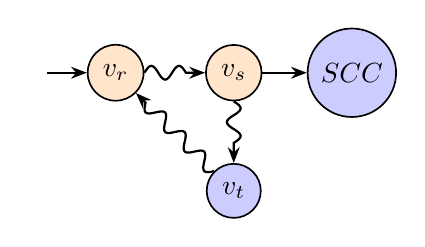
\begin{tikzpicture}[scale=.5,auto=left]
			\node (v0) at (0,0) {};
			\node [circle,draw,semithick,fill=orange!20,radius=0.4] (vr) at (2,0) {$v_r$};
			\node [circle,draw,semithick,fill=orange!20,radius=0.4] (vs) at (5,0) {$v_s$};
			\node [circle,draw,semithick,fill=blue!20,radius=0.4] (vt) at (5,-3) {$v_t$};
			\node [circle,draw,semithick,fill=blue!20,radius=1] (SCC) at (8,0) {$SCC$};
			\draw [-{Stealth[length=2mm]}][black, thick] (v0) -- (vr);
			\draw [decorate,decoration={coil,aspect=0},-{Stealth[length=2mm]}][black, thick] (vr) -- (vs);
			\draw [decorate,decoration={coil,aspect=0},-{Stealth[length=2mm]}][black, thick] (vs) -- (vt);
			\draw [decorate,decoration={coil,aspect=0},-{Stealth[length=2mm]}][black, thick] (vt) -- (vr);
			\draw [-{Stealth[length=2mm]}][black, thick] (vs) -- (SCC);
		\end{tikzpicture}
	\end{center}
	\begin{itemize}
		\item
		Assume the current node is $v_s$ which has at least two adjacent nodes.
		The current path is $P=(\cdots,\,v_r,\,\cdots,\,v_s)$.
		\item
		For the node adjacent to $v_s$ but also in the $SCC$, after running Sub-DFS() on this node, 
		it will be removed with the SCC.
	\end{itemize}
\end{frame}

\begin{frame}{How to implement by DFS?}
	\begin{center}
		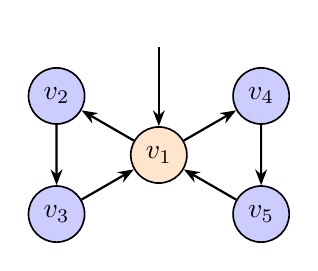
\begin{tikzpicture}[scale=.75,auto=left]
			\node (v0) at (0,2) {};
			\node [circle,draw,semithick,fill=orange!20,radius=0.4] (v1) at (0,0) {$v_1$};
			\node [circle,draw,semithick,fill=blue!20,radius=0.4] (v2) at (-1.732,1) {$v_2$};
			\node [circle,draw,semithick,fill=blue!20,radius=0.4] (v3) at (-1.732,-1) {$v_3$};
			\node [circle,draw,semithick,fill=blue!20,radius=0.4] (v4) at (1.732,1) {$v_4$};
			\node [circle,draw,semithick,fill=blue!20,radius=0.4] (v5) at (1.732,-1) {$v_5$};
			\foreach \from/\to in {v0/v1, v1/v2, v2/v3, v3/v1, v1/v4, v4/v5, v5/v1}
				\draw [-{Stealth[length=2mm]}][black, thick] (\from) -- (\to);
		\end{tikzpicture}
	\end{center}
	\begin{itemize}
		\item
		For nodes in strong components $(v_r,\,\cdots,\,v_s,\,\cdots,\,v_t)$, they cannot be
		deleted(but be contracted first) until the Sub-DFS() on the last vertex $v_r$ in this
		SCC is finished.
	\end{itemize}
\end{frame}

\begin{frame}{Pseudo Code}
	\SetAlFnt{\normalsize}
	\begin{algorithm}[H]
		\caption{Strong components: Main-DFS(G) (DFS caller)}
		$H=G$\;
		\While{$H$ still has a vertex $v$}{
			Sub-DFS(v)\tcc*[l]{start a new path $P = (v)$}
		}
	\end{algorithm}
\end{frame}

\begin{frame}{Pseudo Code}
	\SetAlFnt{\normalsize}
	\begin{algorithm}[H]
		\caption{Strong components: Sub-DFS(v) (DFS callee)}
		add the $v$ as the new last vertex of path $P$\;
		\For{$w\in \{$vertices adjacent to $v\}$}{
			\If{$w\notin P$}{
				Sub-DFS$(w)$\;
			}\Else(\tcc*[h]{$w=v_i$, and $v=v_k$}){
				contract the cycle $v_i,\, v_{i+1},\,\cdots,\,v_k$, both in $H$ and in $P$\;
			}
		}
		\If{no edge leaves $v$ and $v$ is the last DFS-finished vertex in a SCC}{
			output $v$ as a vertex of the strong component graph\;
			delete $v$ from both $H$ and $P$\;
		}
	\end{algorithm}
\end{frame}

\begin{frame}{Assessment}
	\begin{itemize}
		\item
		Note that \emph{contracting} means selecting one vertex as a representation and \alert{merging} others rather than deleting them.
		\item
		Correctness: If no edge leaves $v_k$ then $v_k$ is a vertex of the finest acyclic contraction.
	\end{itemize}
\end{frame}

\begin{frame}{Assessment}
	\begin{itemize}
		\item
		The time consumption of each statement in the pseudo-code is clear. Total time complexity is linear.
		except this statement:
	\end{itemize}
	\begin{center}
		\texttt{\small 
		contract the cycle $v_i,\, v_{i+1},\,\cdots,\,v_k$, both in $H$ and in $P$;
		}
	\end{center}	
	\begin{itemize}
		\item
		Problem is how to merge in linear time while keeping the next time accessing this vertex still in constant time.
		\item
		Therefore, a good data structure for disjoint-set merging is needed usually.
	\end{itemize}
\end{frame}


\subsection{Contribution}

\begin{frame}{Gabow's Contribution}%{Subtitles are optional.}
  % - A title should summarize the slide in an understandable fashion
  %   for anyone how does not follow everything on the slide itself.

	\begin{itemize}
		\item
		He gave a simple list-based implementation that achieves linear time.
		\item
		Use only stacks and arrays as data structure. % Mentioned in introduction.
		\item
		Do not need a disjoint set merging data structure.
	\end{itemize}
\end{frame}

\begin{frame}{Data Structure Used in Algorithm}
	\begin{itemize}
		\item
		In DFS, the \alert{path $P$} from root to each node is almost always significant. So it is in this algorithm.
		\item
		A \alert{stack $S$} contains the sequence of vertices in $P$.
		\item
		A \alert{stack $B$} contains the boundaries between contracted vertices.
		\item
		An array \alert{$I[1\ldots n]$} is used to store stack indices corresponding to vertices.
	\end{itemize}
\end{frame}

\begin{frame}{Contraction Makes Much Difference}
	\begin{itemize}
		\item
		When contraction is executed, some vertices merges into a set.
		\item
		It is possible that several elements in stack $S$ are in the same vertex in path $P$.
		More formal, 
		\begin{center}
			$v_i={S[j]:\, B[i]\leq j< B[i+1]}$
		\end{center}
		\item
		By the way, the formal definition of $I[v]$ is
		\begin{center}
			$I[j]=\begin{cases}
			0, & \text{if }v\text{ has never been in P;} \\
			j, & \text{if }v\text{ is currently in P and }S[j]=v\text{;} \\
			c, & \text{if the strong component containing }v\text{ has}\\
			& \text{been deleted and numbered as }c\text{.}
			\end{cases}$
		\end{center}
		where $c$ counts from $n+1$.
	\end{itemize}
\end{frame}

\begin{frame}[fragile]{New algorithm to discover strong components}
	\SetAlFnt{\normalsize}
	\begin{procedure}[H]
		\caption{STRONG(G)}
		empty stacks $S$ and $B$\;
		\For{$v\in V$}{
			$I[v]=0$\;
		}
		$c=n$\;
		\For{$v\in V$}{
			\If(\tcc*[h]{vertex $v$ has never been accessed yet}){$I[v]=0$}{
				DFS$(v)$\;
			}
		}
	\end{procedure}
\end{frame}

\begin{frame}[fragile]{New algorithm to discover strong components}
	\SetAlFnt{\small}
	\begin{procedure}[H]
		\caption{DFS(v)}
		PUSH$(v,S)$;\quad $I[v]=$TOP$(S)$;\quad PUSH$(I[v],B)$\;
		\tcc{add $v$ to the end of $P$}
		\For{egdes$(v,w)\in E$}{
			\uIf{$I[w]=0$}{
				DFS$(w)$\;
			}\Else(\tcc*[h]{contract if necessary}){
				\While{$I[w]<B[$TOP$(B)]$}{POP$(B)$\;}
			}
		}
		\If(\tcc*[h]{number vertices of the next strong component}){$I[v]=B[$TOP$(B)]$} {
			POP$(B)$\;
			$c = c + 1$\;
			\While{$I[v]\leq $TOP$(S)$}{$I[$POP$(S)]=c$\;}
		}
	\end{procedure}
\end{frame}

\begin{frame}{Demo: Gabow's strong components algorithm}
	\begin{columns}
		\begin{column}{4cm}
			\begin{exampleblock}{Data in memory}
				B and S: stack. I: array. \newline
				\only<1>{
					\mygraphb{}{}{}{}{1/0,2/0,3/0,4/0,5/0,6/0}{
					}
				}
			\end{exampleblock}
		\end{column}
		\begin{column}{5.5cm}
			\begin{exampleblock}{Graph H}
				\only<1>{
					\mygrapha{n1/n2, n1/n3, n2/n3, n2/n4,n4/n3, n4/n5,n5/n2, n5/n6, n6/n3, n6/n4}{}{
					}
				}
			\end{exampleblock}
		\end{column}
	\end{columns}
	\begin{itemize}
		\only<1>{
			\item
			Call Stack: STRONG()
			\item
			This state is the first after initialized. DFS(1) is going to be called.
		}
	\end{itemize}
\end{frame}

\begin{frame}{Demo: Gabow's strong components algorithm}
	\begin{columns}
		\begin{column}{4cm}
			\begin{exampleblock}{Data in memory}
				B and S: stack. I: array. \newline
				\mygraphb{1/1}{}{1/1}{}{1/1,2/0,3/0,4/0,5/0,6/0}{
					
				}
			\end{exampleblock}
		\end{column}
		\begin{column}{5.5cm}
			\begin{exampleblock}{Graph H}
				\mygrapha{n1/n2, n1/n3, n2/n3, n2/n4,n4/n3, n4/n5,n5/n2, n5/n6, n6/n3, n6/n4}{}{
					
				}
			\end{exampleblock}
		\end{column}
	\end{columns}
	\begin{itemize}
		\item
		Call Stack: STRONG()$\rightarrow$DFS(1)
		\item
		Code: \texttt{
			\textbf{for} edges(v,w)$\in$E \textbf{do} ...
		}
		\item
		$w=2$.
	\end{itemize}
\end{frame}

\begin{frame}{Demo: Gabow's strong components algorithm}
	\begin{columns}
		\begin{column}{4cm}
			\begin{exampleblock}{Data in memory}
				B and S: stack. I: array. \newline
				\mygraphb{1/1,2/2}{}{1/1,2/2}{}{1/1,2/2,3/0,4/0,5/0,6/0}{
					
				}
			\end{exampleblock}
		\end{column}
		\begin{column}{5.5cm}
			\begin{exampleblock}{Graph H}
				\mygrapha{n1/n3, n2/n3, n2/n4,n4/n3, n4/n5,n5/n2, n5/n6, n6/n3, n6/n4}{n1/n2}{
					
				}
			\end{exampleblock}
		\end{column}
	\end{columns}
	\begin{itemize}
		\item
		Call Stack: STRONG()$\rightarrow$DFS(1)$\rightarrow$DFS(2)
		\item
		Code: \texttt{
			\textbf{for} edges(v,w)$\in$E \textbf{do} ...
		}
		\item
		$w=3$.
	\end{itemize}
\end{frame}

\begin{frame}{Demo: Gabow's strong components algorithm}
	\begin{columns}
		\begin{column}{4cm}
			\begin{exampleblock}{Data in memory}
				B and S: stack. I: array. \newline
				\mygraphb{1/1,2/2,3/3}{}{1/1,2/2,3/3}{}{1/1,2/2,3/3,4/0,5/0,6/0}{
					
				}
			\end{exampleblock}
		\end{column}
		\begin{column}{5.5cm}
			\begin{exampleblock}{Graph H}
				\mygrapha{n1/n3, n2/n4,n4/n3, n4/n5,n5/n2, n5/n6, n6/n3, n6/n4}{n1/n2, n2/n3}{
					
				}
			\end{exampleblock}
		\end{column}
	\end{columns}
	\begin{itemize}
		\item
		Call Stack: STRONG()$\rightarrow$DFS(1)$\rightarrow$DFS(2)$\rightarrow$DFS(3)
		\item
		Code: \texttt{
			\textbf{if} I[v]$=$B[TOP(B)] \textbf{then} ...
		}
		\item
		Go back.
	\end{itemize}
\end{frame}

\begin{frame}{Demo: Gabow's strong components algorithm}
	\begin{columns}
		\begin{column}{4cm}
			\begin{exampleblock}{Data in memory}
				B and S: stack. I: array. \newline
				\mygraphb{1/1,2/2,3/3}{}{1/1,2/2,3/4}{}{1/1,2/2,3/7,4/3,5/0,6/0}{
					
				}
			\end{exampleblock}
		\end{column}
		\begin{column}{5.5cm}
			\begin{exampleblock}{Graph H}
				\mygrapha{n1/n3, n4/n3, n4/n5,n5/n2, n5/n6, n6/n3, n6/n4, n2/n3}{n1/n2, n2/n4}{
					% component node 3
					\fill [yellow, semitransparent] (6,4) rectangle (8,6);
					% discard node 3
					\draw [thick, red] (6.5, 5.5) -- (7.5, 4.5);
					\draw [thick, red] (6.5, 4.5) -- (7.5, 5.5);
				}
			\end{exampleblock}
		\end{column}
	\end{columns}
	\begin{itemize}
		\item
		Call Stack: STRONG()$\rightarrow$DFS(1)$\rightarrow$DFS(2)$\rightarrow$DFS(4)
		\item
		Code: \texttt{
			\textbf{for} edges(v,w)$\in$E \textbf{do} ...
		}
		\item
		$w=5$.
	\end{itemize}
\end{frame}

\begin{frame}{Demo: Gabow's strong components algorithm}
	\begin{columns}
		\begin{column}{4cm}
			\begin{exampleblock}{Data in memory}
				B and S: stack. I: array. \newline
				\mygraphb{1/1,2/2,3/3,4/4}{}{1/1,2/2,3/4,4/5}{}{1/1,2/2,3/7,4/3,5/4,6/0}{
					
				}
			\end{exampleblock}
		\end{column}
		\begin{column}{5.5cm}
			\begin{exampleblock}{Graph H}
				\mygrapha{n1/n3, n4/n3, n5/n2, n5/n6, n6/n3, n6/n4, n2/n3}{n1/n2, n2/n4, n4/n5}{
					% component node 3
					\fill [yellow, semitransparent] (6,4) rectangle (8,6);
					% discard node 3
					\draw [thick, red] (6.5, 5.5) -- (7.5, 4.5);
					\draw [thick, red] (6.5, 4.5) -- (7.5, 5.5);
				}
			\end{exampleblock}
		\end{column}
	\end{columns}
	\begin{itemize}
		\item
		Call Stack: $\cdots\rightarrow$DFS(1)$\rightarrow$DFS(2)$\rightarrow$DFS(4)$\rightarrow$DFS(5)
		\item
		Code: \texttt{
			\textbf{for} edges(v,w)$\in$E \textbf{do} ...
		}
		\item
		$w=2$.
	\end{itemize}
\end{frame}

\begin{frame}{Demo: Gabow's strong components algorithm}
	\begin{columns}
		\begin{column}{4cm}
			\begin{exampleblock}{Data in memory}
				B and S: stack. I: array. \newline
				\mygraphb{1/1,2/2,3/3,4/4}{}{1/1,2/2,3/4,4/5}{}{1/1,2/2,3/7,4/3,5/4,6/0}{
					
				}
			\end{exampleblock}
		\end{column}
		\begin{column}{5.5cm}
			\begin{exampleblock}{Graph H}
				\mygrapha{n1/n3, n4/n3, n5/n6, n6/n3, n6/n4, n2/n3}{n1/n2, n2/n4, n4/n5, n5/n2}{
					% component node 3
					\fill [yellow, semitransparent] (6,4) rectangle (8,6);
					% discard node 3
					\draw [thick, red] (6.5, 5.5) -- (7.5, 4.5);
					\draw [thick, red] (6.5, 4.5) -- (7.5, 5.5);
				}
			\end{exampleblock}
		\end{column}
	\end{columns}
	\begin{itemize}
		\item
		Call Stack: $\cdots\rightarrow$DFS(1)$\rightarrow$DFS(2)$\rightarrow$DFS(4)$\rightarrow$DFS(5)
		\item
		Code: \texttt{
			\textbf{while} I[w]$ < $B[TOP(B)] \textbf{do} POP(B);
		}
		\item
		Now, $w=2$, contract!
	\end{itemize}
\end{frame}

\begin{frame}{Demo: Gabow's strong components algorithm}
	\begin{columns}
		\begin{column}{4cm}
			\begin{exampleblock}{Data in memory}
				B and S: stack. I: array. \newline
				\mygraphb{1/1,2/2}{}{1/1,2/2,3/4,4/5}{}{1/1,2/2,3/7,4/3,5/4,6/0}{
					
				}
			\end{exampleblock}
		\end{column}
		\begin{column}{5.5cm}
			\begin{exampleblock}{Graph H}
				\mygrapha{n1/n3, n4/n3, n5/n6, n6/n3, n6/n4, n2/n3}{n1/n2, n2/n4, n4/n5, n5/n2}{
					% component node 3
					\fill [yellow, semitransparent] (6,4) rectangle (8,6);
					% discard node 3
					\draw [thick, red] (6.5, 5.5) -- (7.5, 4.5);
					\draw [thick, red] (6.5, 4.5) -- (7.5, 5.5);
				}
			\end{exampleblock}
		\end{column}
	\end{columns}
	\begin{itemize}
		\item
		Call Stack: $\cdots\rightarrow$DFS(1)$\rightarrow$DFS(2)$\rightarrow$DFS(4)$\rightarrow$DFS(5)
		\item
		Code: \texttt{
			\textbf{while} I[w]$ < $B[TOP(B)] \textbf{do} POP(B);
		}
		\item
		Now, $w=2$, contract!
	\end{itemize}
\end{frame}

\begin{frame}{Demo: Gabow's strong components algorithm}
	\begin{columns}
		\begin{column}{4cm}
			\begin{exampleblock}{Data in memory}
				B and S: stack. I: array. \newline
				\mygraphb{1/1,2/2}{}{1/1,2/2,3/4,4/5}{}{1/1,2/2,3/7,4/3,5/4,6/0}{
					
				}
			\end{exampleblock}
		\end{column}
		\begin{column}{5.5cm}
			\begin{exampleblock}{Graph H}
				\mygrapha{n1/n3, n4/n3, n6/n3, n6/n4, n2/n3, n5/n2, n5/n6}{n1/n2, n2/n4, n4/n5}{
					% component node 3
					\fill [yellow, semitransparent] (6,4) rectangle (8,6);
					% discard node 3
					\draw [thick, red] (6.5, 5.5) -- (7.5, 4.5);
					\draw [thick, red] (6.5, 4.5) -- (7.5, 5.5);
					% component nodes 2,4,5
					\fill [yellow, semitransparent] (1,0) -- (0,5) -- (1,7) -- (6,3) -- (3,0) -- cycle;
				}
			\end{exampleblock}
		\end{column}
	\end{columns}
	\begin{itemize}
		\item
		Call Stack: $\cdots\rightarrow$DFS(1)$\rightarrow$DFS(2)$\rightarrow$DFS(4)$\rightarrow$DFS(5)
		\item
		Code: \texttt{
			\textbf{if} I[w]$ =0$ \textbf{then} DFS(w);
		}
		\item
		$w=6$.
	\end{itemize}
\end{frame}

\begin{frame}{Demo: Gabow's strong components algorithm}
	\begin{columns}
		\begin{column}{4cm}
			\begin{exampleblock}{Data in memory}
				B and S: stack. I: array. \newline
				\mygraphb{1/1,2/2,3/5}{}{1/1,2/2,3/4,4/5,5/6}{}{1/1,2/2,3/7,4/3,5/4,6/5}{
					
				}
			\end{exampleblock}
		\end{column}
		\begin{column}{5.5cm}
			\begin{exampleblock}{Graph H}
				\mygrapha{n1/n3, n4/n3, n6/n3, n6/n4, n2/n3, n5/n2}{n1/n2, n2/n4, n4/n5, n5/n6}{
					% component node 3
					\fill [yellow, semitransparent] (6,4) rectangle (8,6);
					% discard node 3
					\draw [thick, red] (6.5, 5.5) -- (7.5, 4.5);
					\draw [thick, red] (6.5, 4.5) -- (7.5, 5.5);
					% component nodes 2,4,5
					\fill [yellow, semitransparent] (1,0) -- (0,5) -- (1,7) -- (6,3) -- (3,0) -- cycle;
				}
			\end{exampleblock}
		\end{column}
	\end{columns}
	\begin{itemize}
		\item
		Call Stack: $\cdots\rightarrow$DFS(2)$\rightarrow$DFS(4)$\rightarrow$DFS(5)$\rightarrow$DFS(6)
		\item
		Code: \texttt{
			\textbf{for} edges(v,w)$\in$E \textbf{do} ...
		}
		\item
		$w=4$.
	\end{itemize}
\end{frame}

\begin{frame}{Demo: Gabow's strong components algorithm}
	\begin{columns}
		\begin{column}{4cm}
			\begin{exampleblock}{Data in memory}
				B and S: stack. I: array. \newline
				\mygraphb{1/1,2/2,3/5}{}{1/1,2/2,3/4,4/5,5/6}{}{1/1,2/2,3/7,4/3,5/4,6/5}{
					
				}
			\end{exampleblock}
		\end{column}
		\begin{column}{5.5cm}
			\begin{exampleblock}{Graph H}
				\mygrapha{n1/n3, n4/n3, n6/n3, n2/n3, n5/n2}{n1/n2, n2/n4, n4/n5, n5/n6, n6/n4}{
					% component node 3
					\fill [yellow, semitransparent] (6,4) rectangle (8,6);
					% discard node 3
					\draw [thick, red] (6.5, 5.5) -- (7.5, 4.5);
					\draw [thick, red] (6.5, 4.5) -- (7.5, 5.5);
					% component nodes 2,4,5
					\fill [yellow, semitransparent] (1,0) -- (0,5) -- (1,7) -- (6,3) -- (3,0) -- cycle;
				}
			\end{exampleblock}
		\end{column}
	\end{columns}
	\begin{itemize}
		\item
		Call Stack: $\cdots\rightarrow$DFS(2)$\rightarrow$DFS(4)$\rightarrow$DFS(5)$\rightarrow$DFS(6)
		\item
		Code: \texttt{
			\textbf{while} I[w]$ < $B[TOP(B)] \textbf{do} POP(B);
		}
		\item
		Now, $w=4$, contract!
	\end{itemize}
\end{frame}

\begin{frame}{Demo: Gabow's strong components algorithm}
	\begin{columns}
		\begin{column}{4cm}
			\begin{exampleblock}{Data in memory}
				B and S: stack. I: array. \newline
				\mygraphb{1/1,2/2}{}{1/1,2/2,3/4,4/5,5/6}{}{1/1,2/2,3/7,4/3,5/4,6/5}{
					
				}
			\end{exampleblock}
		\end{column}
		\begin{column}{5.5cm}
			\begin{exampleblock}{Graph H}
				\mygrapha{n1/n3, n4/n3, n6/n3, n2/n3, n5/n2, n6/n4}{n1/n2, n2/n4, n4/n5, n5/n6}{
					% component node 3
					\fill [yellow, semitransparent] (6,4) rectangle (8,6);
					% discard node 3
					\draw [thick, red] (6.5, 5.5) -- (7.5, 4.5);
					\draw [thick, red] (6.5, 4.5) -- (7.5, 5.5);
					% component nodes 2,4,5,6
					\fill [yellow, semitransparent] (1,0) -- (0,5) -- (1,7) -- (8,0) -- cycle;
				}
			\end{exampleblock}
		\end{column}
	\end{columns}
	\begin{itemize}
		\item
		Call Stack: $\cdots\rightarrow$DFS(2)$\rightarrow$DFS(4)$\rightarrow$DFS(5)$\rightarrow$DFS(6)
		\item
		Code: \texttt{
			\textbf{if} I[v]$=$B[TOP(B)] \textbf{then} ...
		}
		\item
		Go back.
	\end{itemize}
\end{frame}

\begin{frame}{Demo: Gabow's strong components algorithm}
	\begin{columns}
		\begin{column}{4cm}
			\begin{exampleblock}{Data in memory}
				B and S: stack. I: array. \newline
				\mygraphb{1/1,2/2}{}{1/1,2/2,3/4,4/5,5/6}{}{1/1,2/2,3/7,4/3,5/4,6/5}{
					
				}
			\end{exampleblock}
		\end{column}
		\begin{column}{5.5cm}
			\begin{exampleblock}{Graph H}
				\mygrapha{n1/n3, n4/n3, n6/n3, n2/n3, n5/n2, n6/n4, n5/n6}{n1/n2, n2/n4, n4/n5}{
					% component node 3
					\fill [yellow, semitransparent] (6,4) rectangle (8,6);
					% discard node 3
					\draw [thick, red] (6.5, 5.5) -- (7.5, 4.5);
					\draw [thick, red] (6.5, 4.5) -- (7.5, 5.5);
					% component nodes 2,4,5,6
					\fill [yellow, semitransparent] (1,0) -- (0,5) -- (1,7) -- (8,0) -- cycle;
				}
			\end{exampleblock}
		\end{column}
	\end{columns}
	\begin{itemize}
		\item
		Call Stack: $\cdots\rightarrow$DFS(2)$\rightarrow$DFS(4)$\rightarrow$DFS(5)
		\item
		Code: \texttt{
			\textbf{if} I[v]$=$B[TOP(B)] \textbf{then} ...
		}
		\item
		Go back.
	\end{itemize}
\end{frame}

\begin{frame}{Demo: Gabow's strong components algorithm}
	\begin{columns}
		\begin{column}{4cm}
			\begin{exampleblock}{Data in memory}
				B and S: stack. I: array. \newline
				\mygraphb{1/1,2/2}{}{1/1,2/2,3/4,4/5,5/6}{}{1/1,2/2,3/7,4/3,5/4,6/5}{
					
				}
			\end{exampleblock}
		\end{column}
		\begin{column}{5.5cm}
			\begin{exampleblock}{Graph H}
				\mygrapha{n1/n3, n4/n3, n6/n3, n2/n3, n5/n2, n6/n4, n5/n6, n4/n5}{n1/n2, n2/n4}{
					% component node 3
					\fill [yellow, semitransparent] (6,4) rectangle (8,6);
					% discard node 3
					\draw [thick, red] (6.5, 5.5) -- (7.5, 4.5);
					\draw [thick, red] (6.5, 4.5) -- (7.5, 5.5);
					% component nodes 2,4,5,6
					\fill [yellow, semitransparent] (1,0) -- (0,5) -- (1,7) -- (8,0) -- cycle;
				}
			\end{exampleblock}
		\end{column}
	\end{columns}
	\begin{itemize}
		\item
		Call Stack: $\cdots\rightarrow$DFS(2)$\rightarrow$DFS(4)
		\item
		Code: \texttt{
			\textbf{if} I[v]$=$B[TOP(B)] \textbf{then} ...
		}
		\item
		Go back.
	\end{itemize}
\end{frame}

\begin{frame}{Demo: Gabow's strong components algorithm}
	\begin{columns}
		\begin{column}{4cm}
			\begin{exampleblock}{Data in memory}
				B and S: stack. I: array. \newline
				\mygraphb{1/1,2/2}{}{1/1,2/2,3/4,4/5,5/6}{}{1/1,2/2,3/7,4/3,5/4,6/5}{
					
				}
			\end{exampleblock}
		\end{column}
		\begin{column}{5.5cm}
			\begin{exampleblock}{Graph H}
				\mygrapha{n1/n3, n4/n3, n6/n3, n2/n3, n5/n2, n6/n4, n5/n6, n4/n5, n2/n4}{n1/n2}{
					% component node 3
					\fill [yellow, semitransparent] (6,4) rectangle (8,6);
					% discard node 3
					\draw [thick, red] (6.5, 5.5) -- (7.5, 4.5);
					\draw [thick, red] (6.5, 4.5) -- (7.5, 5.5);
					% component nodes 2,4,5,6
					\fill [yellow, semitransparent] (1,0) -- (0,5) -- (1,7) -- (8,0) -- cycle;
				}
			\end{exampleblock}
		\end{column}
	\end{columns}
	\begin{itemize}
		\item
		Call Stack: STRONG()$\rightarrow$DFS(1)$\rightarrow$DFS(2)
		\item
		Code: \texttt{
			\textbf{if} I[v]$=$B[TOP(B)] \textbf{then} ...
		}
		\item
		Go back. But this time, \alert{Condition in last line is satisfied!}
	\end{itemize}
\end{frame}

\begin{frame}{Demo: Gabow's strong components algorithm}
	\begin{columns}
		\begin{column}{4cm}
			\begin{exampleblock}{Data in memory}
				B and S: stack. I: array. \newline
				\mygraphb{1/1}{}{1/1}{}{1/1,2/8,3/7,4/8,5/8,6/8}{
					
				}
			\end{exampleblock}
		\end{column}
		\begin{column}{5.5cm}
			\begin{exampleblock}{Graph H}
				\mygrapha{n1/n3, n4/n3, n6/n3, n2/n3, n5/n2, n6/n4, n5/n6, n4/n5, n2/n4}{n1/n2}{
					% component node 3
					\fill [yellow, semitransparent] (6,4) rectangle (8,6);
					% discard node 3
					\draw [thick, red] (6.5, 5.5) -- (7.5, 4.5);
					\draw [thick, red] (6.5, 4.5) -- (7.5, 5.5);
					% component nodes 2,4,5,6
					\fill [yellow, semitransparent] (1,0) -- (0,5) -- (1,7) -- (8,0) -- cycle;
					% discard nodes 2,4,5,6
					\draw [thick, red] (0.5, 5.5) -- (1.5, 4.5);
					\draw [thick, red] (0.5, 4.5) -- (1.5, 5.5);
					\draw [thick, red] (3.5, 3.5) -- (4.5, 2.5);
					\draw [thick, red] (3.5, 2.5) -- (4.5, 3.5);
					\draw [thick, red] (1.5, 1.5) -- (2.5, 0.5);
					\draw [thick, red] (1.5, 0.5) -- (2.5, 1.5);
					\draw [thick, red] (5.5, 1.5) -- (6.5, 0.5);
					\draw [thick, red] (5.5, 0.5) -- (6.5, 1.5);
				}
			\end{exampleblock}
		\end{column}
	\end{columns}
	\begin{itemize}
		\item
		Call Stack: STRONG()$\rightarrow$DFS(1)$\rightarrow$DFS(2)
		\item
		Code: \texttt{
			\textbf{while} I[v]$\leq$TOP(S) \textbf{do} I[POP(S)]=c;
		}
		\item
		Pop 2 from B, while 2, 4, 5, 6 in S are also popped.
	\end{itemize}
\end{frame}

\begin{frame}{Demo: Gabow's strong components algorithm}
	\begin{columns}
		\begin{column}{4cm}
			\begin{exampleblock}{Data in memory}
				B and S: stack. I: array. \newline
				\mygraphb{}{}{}{}{1/9,2/8,3/7,4/8,5/8,6/8}{
					
				}
			\end{exampleblock}
		\end{column}
		\begin{column}{5.5cm}
			\begin{exampleblock}{Graph H}
				\mygrapha{n1/n3, n4/n3, n6/n3, n2/n3, n5/n2, n6/n4, n5/n6, n4/n5, n2/n4, n1/n2}{}{
					% component node 3
					\fill [yellow, semitransparent] (6,4) rectangle (8,6);
					% discard node 3
					\draw [thick, red] (6.5, 5.5) -- (7.5, 4.5);
					\draw [thick, red] (6.5, 4.5) -- (7.5, 5.5);
					% component nodes 2,4,5,6
					\fill [yellow, semitransparent] (1,0) -- (0,5) -- (1,7) -- (8,0) -- cycle;
					% discard nodes 2,4,5,6
					\draw [thick, red] (0.5, 5.5) -- (1.5, 4.5);
					\draw [thick, red] (0.5, 4.5) -- (1.5, 5.5);
					\draw [thick, red] (3.5, 3.5) -- (4.5, 2.5);
					\draw [thick, red] (3.5, 2.5) -- (4.5, 3.5);
					\draw [thick, red] (1.5, 1.5) -- (2.5, 0.5);
					\draw [thick, red] (1.5, 0.5) -- (2.5, 1.5);
					\draw [thick, red] (5.5, 1.5) -- (6.5, 0.5);
					\draw [thick, red] (5.5, 0.5) -- (6.5, 1.5);
					% discard node 1
					\draw [thick, red] (3.5, 7.5) -- (4.5, 6.5);
					\draw [thick, red] (3.5, 6.5) -- (4.5, 7.5);
					% component node 1
					\fill [yellow, semitransparent] (3,6) rectangle (5,8);
				}
			\end{exampleblock}
		\end{column}
	\end{columns}
	\begin{itemize}
		\item
		Call Stack: STRONG()$\rightarrow$DFS(1)
		\item
		Code: \texttt{
			\textbf{while} I[v]$\leq$TOP(S) \textbf{do} I[POP(S)]=c;
		}
		\item
		Pop the last one both in B and in S. \emph{Finished!!}
	\end{itemize}
\end{frame}


\subsection{Discussion}

\begin{frame}{Correctness of Gabow's Strong Components Algorithm}
	\begin{theorem}[Correctness and Time Complexity]
		When STRONG(G) halts each vertex $v\in V$ belongs to the strong component numbered $I[v]$.
		The time and space are both $O(V+E)$.
	\end{theorem}
	\begin{itemize}
		\item
		The key of proof is to show that STRONG(G) is a valid implementation of the P\&M's high-level algorithm.
	\end{itemize}
\end{frame}

\begin{frame}{Framework of STRONG(G)}
	\SetAlFnt{\small}
	\begin{algorithm}[H]
		\caption{Strong components: Main-DFS(G) (DFS caller)}
		$H=G$\;
		\While{$H$ still has a vertex $v$}{
			Sub-DFS(v)\tcc*[l]{start a new path $P = (v)$}
		}
	\end{algorithm}
	\begin{procedure}[H]
		\caption{STRONG(G)}
		empty stacks $S$ and $B$\;
		\For{$v\in V$}{
			$I[v]=0$\;
		}
		$c=n$\;
		\For{$v\in V$}{
			\If(\tcc*[h]{$v$ has never been accessed}){$I[v]=0$}{
				DFS$(v)$\;
			}
		}
	\end{procedure}
\end{frame}

\begin{frame}{Growing Path P}
	\SetAlFnt{\small}
	\begin{algorithm}[H]
		\caption{A Part of High-Level Algorithm}
		\For{$w\in \{$vertices adjacent to $v\}$}{
			\If{$w\notin P$}{
				Sub-DFS$(w)$\;
			}\Else(\tcc*[h]{$w=v_i$, and $v=v_k$}){
				contract the cycle $v_i,\, v_{i+1},\,\cdots,\,v_k$, both in $H$ and in $P$\;
			}
		}
	\end{algorithm}
	\begin{procedure}[H]
		\caption{A Part of DFS(v)}
		\For{egdes$(v,w)\in E$}{
			\uIf{$I[w]=0$}{
				DFS$(w)$\;
			}\Else(\tcc*[h]{contract if necessary}){
				\While{$I[w]<B[$TOP$(B)]$}{POP$(B)$\;}
			}
		}
	\end{procedure}
\end{frame}

\begin{frame}{Having Found a Strong Components}
	\SetAlFnt{\small}
	\begin{algorithm}[H]
		\caption{A Part of High-Level Algorithm}
		\If{no edge leaves $v$ and $v$ is the last DFS-finished vertex in a SCC}{
			output $v$ as a vertex of the strong component graph\;
			delete $v$ from both $H$ and $P$\;
		}
	\end{algorithm}
	\begin{procedure}[H]
		\caption{A Part of DFS(v)}
		\If(\tcc*[h]{number vertices of the next strong component}){$I[v]=B[$TOP$(B)]$} {
			POP$(B)$\;
			$c = c + 1$\;
			\While{$I[v]\leq $TOP$(S)$}{$I[$POP$(S)]=c$\;}
		}
	\end{procedure}
\end{frame}

\begin{frame}{Time Complexity}
	\begin{itemize}
		\item
		Every vertex is pushed onto and popped from each stack $S$, $B$ exactly once.
		So the algorithm spends $O(1)$ time on each vertex or edge.
		\item
		Time Complexity: $O(V+E)$
		\item
		Intuitively, from another view, this algorithm is based on DFS, and no loop
		is executed on one vertex or one edge.
	\end{itemize}
\end{frame}



\section{Biconnected Components}

\subsection{Review}

\begin{frame}{Review: Biconnected Component}
	\begin{itemize}
		\item
		A \emph{biconnected component} of G is a maximal set of edges such that any
		two edges in the set lie on a common simple cycle.		
	\end{itemize}
	\begin{center}
		\includegraphics<1>[height=3cm]{biconnected_0.png}%
	\end{center}
\end{frame}

\subsection{High-Level Algorithm}

\begin{frame}{Concepts: Hypergraph}
	\begin{itemize}
		\item
		A \emph{hypergraph} $H=(V,E)$ is a generalization of a graph in which
		an edge can join any number of vertices.
		\item
		In the following hypergraph, 
	\end{itemize}
	\begin{center}
		$V = \{v_1, v_2, v_3, v_4, v_5, v_6, v_7\}$
		\begin{align*}
			E &= \{e_1,e_2,e_3,e_4\}\\
			&= \{\{v_1,v_2,v_3\},\{v_2,v_3\},\{v_3,v_5,v_6\},\{v_4\}\}
		\end{align*}
		\includegraphics<1>[height=3cm]{hypergraph_0.png}%
	\end{center}
\end{frame}

\begin{frame}{Concepts: Hypergraph}
	\begin{itemize}
		\item
		Therefore, we need redefine the \emph{edge}, \emph{path}, \emph{cycle}, $\cdots$, 
		and nearly all concepts as long as it is relative to edge.
		\item
		A \emph{path} is a sequence $(v_1, e_1, \cdots, v_k, e_k)$ of distinct vertices
		$v_i$ and distinct edges $e_i$, $1\leq i\leq k$, with $v_1\in e_1$ and $v_i\in e_{i-1}\cap e_i$
		for every $1 < i\leq k$.
		\item
		An important property:
		$$v_{i+1}\in e_i-v_i, \quad 1\leq i < k$$
		\item
		Merging a set of edges is to replace old edges with the new one:
		$$e_{new}=\bigcup_{i=1}^ke_i$$
	\end{itemize}
\end{frame}

\begin{frame}{Addtional Concepts We Need}
	\begin{itemize}
		\item
		The \emph{block hypergraph} $H$ of $G$ is the hypergraph formed by merging the edges of each biconnected component of $G$.
		\item
		The set of all vertices in edges of $P$ is denoted
		\begin{center}
			$V(P)=\bigcup_{i=1}^ke_i$
		\end{center}
	\end{itemize}
\end{frame}

\begin{frame}{High-Level Algorithm in Plain Text}
	\begin{itemize}
		\item
		Initially $H$ is the given graph $G$. If $H$ has no edges stop. Otherwise start a new path $P$ by choosing an edge 
		$\{v,\,w\}$ and setting $P=(v,\,\{v,\,w\})$. Continue by growing $P$.
		\item
		To grow the path $P=(v_1,\,e_1,\,\cdots,\,v_k,\,e_k)$ choose an edge $\{v,\,w\}\neq e_k$ with $v\in e_k-v_k$ and do:
		\begin{itemize}
			\item
			If $w\notin V(P)$, add $v,\,\{v,\,w\}$ to the end of $P$. Continue growing $P$.
			\item
			If $w\in V(P)$, say $w\in e_i-v_{i+1}$, merge the edges of the cycle $w,\,e_i,\,v_{i+1},\,e_{i+1},\,\cdots,\,v_k,\,e_k,\,v,\,\{v,\,w\}$
			to a new edge $e=\bigcup_{j=i}^ke_j$, both in $H$ and in $P$. Continue growing $P$.
			\item
			If no edge leaves $e_k-v_k$, output $e_k$ as an edge of the block hypergraph. Delete $e_k$ from $H$ and delete $(v_k,\,e_k)$
			from $P$. If $P$ is now nonempty continue growing $P$. Otherwise try to start a new path $P$.
		\end{itemize}
	\end{itemize}
\end{frame}

\begin{frame}{Pseudo Code}
	\SetAlFnt{\small}
	\begin{algorithm}[H]
		\caption{Biconnected Components}
		$H=G$\;
		\While{$H$ still has an edge $\{v,w\}$}{
			start a new path $P = (v,\{v,w\})$\;
			\While(\tcc*[h]{Grows path $P$}){$P$ is not empty}{ % TODO
				\If{the last vertex $v_k$ of $P$ has an edge $(v_k, w)$ }{
					\If(\tcc*[h]{$V\{P\}$ is the set of all vertices in $P$}){$w\notin V{P}$}{
						add $v,\{v,w\}$ to the end of $P$, as the new last vertex and edge of $P$\;
					}\Else(\tcc*[h]{$w\in e_i-v_{i+1}$, but most likely $w\neq v_i$}){
						replace the cycle $w,\,e_i,\,v_{i+1},\,e_{i+1},\,\cdots,\,v_k,\,e_k,\,v,\,\{v,\,w\}$
						to a new edge $e=\bigcup_{j=i}^ke_j$, both in $H$ and in $P$\;
					}
				}\Else{
					output $v_k$ as a vertex of the strong component graph\;
					delete $v_k$ from both $H$ and $P$\;
				}
			}
		}
	\end{algorithm}
\end{frame}

\subsection{Gabow's Algorithms}

\begin{frame}{Algorithms}
	\SetAlFnt{\normalsize}
	\begin{procedure}[H]
		\caption{BICONN(G)}
		empty stacks $S$ and B\;
		\For{$v\in V$}{
			$I[v]=0$\;
		}
		$c=n$\;
		\For{$v\in V$}{
			\If{$I[v]=0$ and $v$ is not isolated}{
				DFS$(v)$\;
			}
		}
	\end{procedure}
\end{frame}

\begin{frame}{Algorithms}
	\SetAlFnt{\small}
	\begin{procedure}[H]
		\caption{DFS(v)}
		PUSH$(v,S)$;\quad $I[v]=$TOP$(S)$\;
		\If(\tcc*[h]{create a filled arrow on $B$}){$I[v] > 1$}{
			PUSH$(I[v],B)$\;
		}
		\For{egdes$\{v,w\}\in E$}{
			\uIf(\tcc*[h]{create an open arrow on $B$}){$I[w]=0$}{
				PUSH$(I[v],B)$;\quad DFS$(w)$\;
			}\Else(\tcc*[h]{possible merge}){
				\While{$I[v]>1$ and $I[w]<B[$TOP$(B)-1]$}{POP$(B)$;\quad POP$(B)$\;}
			}
		}
		\uIf{$I[v]=1$}{$I[$POP$(S)]=c$\;}
		\ElseIf{$I[v]=B[$TOP$(B)]$} {
			POP$(B)$;\quad POP$(B)$;\quad $c = c + 1$\;
			\lWhile{$I[v]\leq $TOP$(S)$}{$I[$POP$(S)]=c$}
		}
	\end{procedure}
\end{frame}

\begin{frame}{Demo: Gabow's biconnected components algorithm}
	\begin{columns}
		\begin{column}{4cm}
			\begin{exampleblock}{Data in memory}
				B and S: stack. I: array. \newline
				\only<1>{
					\mygraphd{}{}{}{}{1/0,2/0,3/0,4/0,5/0,6/0,7/0}{
						\myarrowa{}{}
					}
				}
				\only<2>{
					\mygraphd{1/1}{}{1/1}{}{1/1,2/0,3/0,4/0,5/0,6/0,7/0}{
						\myarrowa{}{1}
					}
				}
				\only<3>{
					\mygraphd{1/1,2/2,3/2}{}{1/1,2/2}{}{1/1,2/2,3/0,4/0,5/0,6/0,7/0}{
						\myarrowa{2}{1,2}
					}
				}
				\only<4>{
					\mygraphd{1/1,2/2}{}{1/1,2/2,3/3}{}{1/1,2/2,3/3,4/0,5/0,6/0,7/0}{
						\myarrowa{2}{1}
					}
				}
				\only<5>{
					\mygraphd{1/1,2/2,3/3}{}{1/1,2/2,3/3}{}{1/1,2/2,3/3,4/0,5/0,6/0,7/0}{
						\myarrowa{2}{1,3}
					}
				}
				\only<6>{
					\mygraphd{1/1,2/2}{}{1/1,2/2,3/3,4/4}{}{1/1,2/2,3/3,4/4,5/0,6/0,7/0}{
						\myarrowa{2}{1}
					}
				}
				\only<7>{
					\mygraphd{1/1,2/2,3/4}{}{1/1,2/2,3/3,4/4}{}{1/1,2/2,3/3,4/4,5/0,6/0,7/0}{
						\myarrowa{2}{1,4}
					}
				}
				\only<8>{
					\mygraphd{1/1,2/2}{}{1/1,2/2,3/3,4/4,5/5}{}{1/1,2/2,3/3,4/4,5/5,6/0,7/0}{
						\myarrowa{2}{1}
					}
				}
				\only<9>{
					\mygraphd{1/1,2/2,3/5}{}{1/1,2/2,3/3,4/4,5/5}{}{1/1,2/2,3/3,4/4,5/5,6/0,7/0}{
						\myarrowa{2}{1,5}
					}
				}
				\only<10>{
					\mygraphd{1/1,2/2,3/5,4/6,5/6}{}{1/1,2/2,3/3,4/4,5/5,6/6}{}{1/1,2/2,3/3,4/4,5/5,6/6,7/0}{
						\myarrowa{2,6}{1,5,6}
					}
				}
				\only<11>{
					\mygraphd{1/1,2/2,3/5,4/6}{}{1/1,2/2,3/3,4/4,5/5,6/6,7/7}{}{1/1,2/2,3/3,4/4,5/5,6/6,7/7}{
						\myarrowa{2,6}{1,5}
					}
				}
				\only<12>{
					\mygraphd{1/1,2/2,3/5,4/6}{}{1/1,2/2,3/3,4/4,5/5,6/6,7/7}{}{1/1,2/2,3/3,4/4,5/5,6/6,7/7}{
						\myarrowa{2,6}{1,5}
					}
				}
				\only<13>{
					\mygraphd{1/1,2/2}{}{1/1,2/2,3/3,4/4,5/5}{}{1/1,2/2,3/3,4/4,5/5,6/8,7/8}{
						\myarrowa{2}{1}
					}
				}
				\only<14>{
					\mygraphd{1/1,2/2}{}{1/1,2/2,3/3,4/4,5/5}{}{1/1,2/2,3/3,4/4,5/5,6/8,7/8}{
						\myarrowa{2}{1}
					}
				}
				\only<15>{
					\mygraphd{1/1,2/2}{}{1/1,2/2,3/3,4/4,5/5}{}{1/1,2/2,3/3,4/4,5/5,6/8,7/8}{
						\myarrowa{2}{1}
					}
				}
				\only<16>{
					\mygraphd{1/1,2/2}{}{1/1,2/2,3/3,4/4,5/5}{}{1/1,2/2,3/3,4/4,5/5,6/8,7/8}{
						\myarrowa{2}{1}
					}
				}
				\only<17>{
					\mygraphd{}{}{1/1}{}{1/1,2/9,3/9,4/9,5/9,6/8,7/8}{
						\myarrowa{}{}
					}
				}
				\only<18>{
					\mygraphd{}{}{}{}{1/9,2/9,3/9,4/9,5/9,6/8,7/8}{
						\myarrowa{}{}
					}
				}
			\end{exampleblock}
		\end{column}
		\begin{column}{5.5cm}
			\begin{exampleblock}{Graph}
				\only<1>{
					\mygraphc{n1/n2, n1/n3, n2/n3, n2/n4, n3/n4, n3/n5, n4/n5, n5/n6, n5/n7, n6/n7}{}{
					}
				}
				\only<2>{
					\mygraphc{n1/n3, n2/n3, n2/n4, n3/n4, n3/n5, n4/n5, n5/n6, n5/n7, n6/n7}{n1/n2}{
					}
				}
				\only<3>{
					\mygraphc{n1/n3, n2/n4, n3/n4, n3/n5, n4/n5, n5/n6, n5/n7, n6/n7}{n1/n2, n2/n3}{
					}
				}
				\only<4>{
					\mygraphc{n2/n4, n3/n4, n3/n5, n4/n5, n5/n6, n5/n7, n6/n7}{n1/n2, n2/n3, n1/n3}{
					}
				}
				\only<5>{
					\mygraphc{n1/n3, n2/n4, n3/n5, n4/n5, n5/n6, n5/n7, n6/n7}{n1/n2, n2/n3, n3/n4}{
					}
				}
				\only<6>{
					\mygraphc{n1/n3, n3/n5, n4/n5, n5/n6, n5/n7, n6/n7}{n1/n2, n2/n3, n3/n4, n2/n4}{
					}
				}
				\only<7>{
					\mygraphc{n1/n3, n2/n4, n3/n5, n5/n6, n5/n7, n6/n7}{n1/n2, n2/n3, n3/n4, n4/n5}{
					}
				}
				\only<8>{
					\mygraphc{n1/n3, n2/n4, n3/n5, n5/n6, n5/n7, n6/n7}{n1/n2, n2/n3, n3/n4, n4/n5}{
					}
				}
				\only<9>{
					\mygraphc{n1/n3, n2/n4, n3/n5, n5/n7, n6/n7}{n1/n2, n2/n3, n3/n4, n4/n5, n5/n6}{
					}
				}
				\only<10>{
					\mygraphc{n1/n3, n2/n4, n3/n5, n5/n7}{n1/n2, n2/n3, n3/n4, n4/n5, n5/n6, n6/n7}{
					}
				}
				\only<11>{
					\mygraphc{n1/n3, n2/n4, n3/n5}{n1/n2, n2/n3, n3/n4, n4/n5, n5/n6, n6/n7, n5/n7}{
					}
				}
				\only<12>{
					\mygraphc{n1/n3, n2/n4, n3/n5, n5/n7}{n1/n2, n2/n3, n3/n4, n4/n5, n5/n6, n6/n7}{
					}
				}
				\only<13>{
					\mygraphc{n1/n3, n2/n4, n3/n5, n5/n7, n6/n7}{n1/n2, n2/n3, n3/n4, n4/n5, n5/n6}{
					}
				}
				\only<14>{
					\mygraphc{n1/n3, n2/n4, n3/n5, n5/n6, n5/n7, n6/n7}{n1/n2, n2/n3, n3/n4, n4/n5}{
					}
				}
				\only<15>{
					\mygraphc{n1/n3, n2/n4, n3/n5, n4/n5, n5/n6, n5/n7, n6/n7}{n1/n2, n2/n3, n3/n4}{
					}
				}
				\only<16>{
					\mygraphc{n1/n3, n2/n4, n3/n4, n3/n5, n4/n5, n5/n6, n5/n7, n6/n7}{n1/n2, n2/n3}{
					}
				}
				\only<17>{
					\mygraphc{n1/n3, n2/n3, n2/n4, n3/n4, n3/n5, n4/n5, n5/n6, n5/n7, n6/n7}{n1/n2}{
					}
				}
				\only<18>{
					\mygraphc{n1/n2, n1/n3, n2/n3, n2/n4, n3/n4, n3/n5, n4/n5, n5/n6, n5/n7, n6/n7}{}{
					}
				}
				% \draw [yellow, semitransparent, line width=10] (1,1) -- (5,1) -- (5,5) -- (1,5) -- cycle;
			\end{exampleblock}
		\end{column}
	\end{columns}
	\begin{itemize}
		\item
		Current procedure:
		\only<1>{BICONN(G)}
		\only<2>{DFS(1): w=2}
		\only<3>{DFS(2): w=3}
		\only<4>{DFS(3): w=1}
		\only<5>{DFS(3): w=4}
		\only<6>{DFS(4): w=2}
		\only<7>{DFS(4): w=5}
		\only<8>{DFS(5): w=3}
		\only<9>{DFS(5): w=6}
		\only<10>{DFS(6): w=7}
		\only<11>{DFS(7): w=5}
		\only<12>{DFS(7): End}
		\only<13>{DFS(6): End}
		\only<14>{DFS(5): End(No operation when w=7)}
		\only<15>{DFS(4): End}
		\only<16>{DFS(3): End(No operation when w=5)}
		\only<17>{DFS(2): End}
		\only<18>{DFS(1): End}
	\end{itemize}
\end{frame}

\section*{Summary}

\begin{frame}{Summary}
	% Keep the summary *very short*.
	\begin{itemize}
		\item
		Gabow gave algorithms to find the strong components and biconnected components more effectively.
		They are one-pass algorithms while do not need a disjoint-set data structure.
		\item
		There is a close relationship between strong components and biconnected components, like two faces of a coin:
		one is directed graph, another is undirected graph.
	\end{itemize}
\end{frame}




% All of the following is optional and typically not needed.
% \appendix
% \section<presentation>*{\appendixname}
% \subsection<presentation>*{For Further Reading}

% \begin{frame}[allowframebreaks]
  % \frametitle<presentation>{For Further Reading}

  % \begin{thebibliography}{10}

  % \beamertemplatebookbibitems
  % Start with overview books.

  % \bibitem{Author1990}
    % A.~Author.
    % \newblock {\em Handbook of Everything}.
    % \newblock Some Press, 1990.


  % \beamertemplatearticlebibitems
  % Followed by interesting articles. Keep the list short.

  % \bibitem{Someone2000}
    % S.~Someone.
    % \newblock On this and that.
    % \newblock {\em Journal of This and That}, 2(1):50--100,
    % 2000.
  % \end{thebibliography}
% \end{frame}

\end{document}
